\documentclass[14pt,aspectratio=169,hyperref={pdftex,unicode},xcolor=dvipsnames]{beamer}
\usepackage[english,russian]{babel}
\usepackage[utf8x]{inputenc}
\usepackage[T2A]{fontenc}
\usepackage{cmap}
\usepackage{paratype}
\usepackage{minted} % для примеров кода (требует параметра -shell-escape)
\usepackage{svg}
% \usepackage{pdfpages}
% \usepackage[pdftex]{graphicx}


\usetheme{metropolis}
\usefonttheme[]{professionalfonts}  % запрещаем beamer'у перезаписывать мат. шрифты
\metroset{numbering=fraction}
\metroset{subsectionpage=progressbar}

\setbeamercolor{frametitle}{fg=black}
\setbeamertemplate{frametitle}
{
 \vspace{3mm}\insertframetitle\par
}
\setbeamertemplate{title separator}{}
\setbeamertemplate{footnote separator}{}


\usebackgroundtemplate{
\includegraphics[width=\paperwidth,height=\paperheight]{./common/background_white.jpg}}

\logo{\vspace{-1.2cm}
\includegraphics[width=6mm]{./common/short-v.pdf}\hspace*{1.08\textwidth}}

\institute
{
  \begin{columns}
    \begin{column}{1.5cm}
    
\includegraphics[height=15mm,keepaspectratio]{./common/math-cs.pdf}
    \end{column}
    \begin{column}{4cm}
          Факультет математики и компьютерных наук СПбГУ
    \end{column}
  \end{columns}
}


\begin{document}

\begin{frame}[plain]
    \begin{center}
        \textbf{Никита Босов}

        {\Large\textbf{Тема работы: расширяемый генератор синтаксически корректных программ для
                обучения программированию}}

        Выпускная квалификационная работа

        {\small Научный руководитель: М.\,М.\,Заславский}

        15 июня 2022
    \end{center}


    \begin{columns}
        \begin{column}{1cm}
            
\includegraphics[height=15mm,keepaspectratio]{./common/math-cs.pdf}
        \end{column}
        \begin{column}{10cm}
            \small
            Факультет математики и~компьютерных наук СПбГУ\\
            Программа <<Современное программирование>>
        \end{column}
    \end{columns}
\end{frame}



\begin{frame}
    \frametitle{Цель дипломной работы}

    \begin{itemize}
        \item На сегодняшний день существует множество курсов по обучению языкам программирования.
        \item Одни из самых популярных задач в таких курсах~--- задачи вида <<что выведет данный код>>.
        \item Для таких задач на сегодняшний день необходимо писать самому или искать примеры программ.
        \item Цель проекта~--- создать генератор таких программ.
    \end{itemize}
\end{frame}

\begin{frame}
    \frametitle{Генераторы программ}
    \begin{itemize}
        \item Генератор программ~--- программа, генерирующая программный код согласно некоторым условиям.
        \item Генераторы программ существуют достаточно давно, однако используются в основном для тестирования
              компиляторов и интерпретаторов.
    \end{itemize}
\end{frame}

\begin{frame}
    \frametitle{Аналоги}
    \begin{itemize}
        \item Программы, используемые для тестирования компиляторов: Csmith, Yarpgen.
        \item Deepsmith~--- инструмент генерации кода на OpenCL, использующий машинное обучение.
    \end{itemize}
\end{frame}

\begin{frame}
    \frametitle{Постановка задачи}
    Разработать генератор обучающих примеров программ в виде текста или изображения с поддержкой
    генерации кода на разных языках программирования и управления задачами, на основе
    которых генерируется код.
\end{frame}


\begin{frame}
    \frametitle{Схема генерации программ}
    \begin{center}
        
\includegraphics[width=\textwidth]{images/generation-steps.drawio.png}
    \end{center}
\end{frame}



\begin{frame}
    \frametitle{Подзадачи}
    \begin{enumerate}
        \item Разработка универсального представления сгенерированных программ (IR), которое можно
              преобразовывать в код на разных языках программирования. Также разработать представление шаблонов,
              которые можно сохранять в базу данных и преобразовывать в IR при подстановке параметров.
        \item Разработка предметно-ориентированного языка построения шаблонов программ.
    \end{enumerate}
\end{frame}

\begin{frame}
    \frametitle{Подзадачи}
    \begin{enumerate}
        \setcounter{enumi}{2}
        \item Добавить возможность добавления и удаления шаблонов.
        \item Добавить возможность генерации изображения программного кода.
        \item Добавить возможность проверки ответов студентов.
    \end{enumerate}
\end{frame}

% \begin{frame}{Задача 1: формула с пояснениями}
%     \small
%     Фильтр минимизирует среднеквадратическое отклонение цвета пикселя.

%     \begin{equation*}\label{eq:wiener_nsr}
%         \hat{Y}(i, j) = \left[ \frac{\hat{H}^*(i, j)}{\left|\hat{H}(i, j)\right|^2 + \frac{S_n(i, j)}{S_s(i, j)}} \right] \times \hat{F}(i, j),
%     \end{equation*}
%     \begin{itemize}
%         \item $Y$ -- восстановленное изображение,  $F$ -- наблюдаемое изображение,
%         \item $H$ -- функция рассеивания, $H^*$ --комплексное сопряжение $H$,
%         \item $S_n$ -- энергетический спектр шума -- $\left| \hat{N} \right|^2$,
%         \item $S_s$ -- энергетический спектр исходного изображения -- $\left| \hat{F} \right|^2$,
%         \item $\times$ -- умножение комплексных чисел.
%     \end{itemize}
% \end{frame}


\begin{frame}
    \frametitle{Архитектура проекта и используемые технологии}
    \begin{itemize}
        \item Веб-сервер~--- фреймворк \texttt{Ktor}
        \item Преобразование шаблонов кода в JSON~--- библиотека \texttt{Kotlinx.serialization}
        \item База данных~--- \texttt{MongoDB}
        \item Генерация изображений кода~--- библиотека \texttt{python-pygments}
    \end{itemize}
\end{frame}

\begin{frame}
    \frametitle{Схема архитектуры проекта}
    \begin{center}
        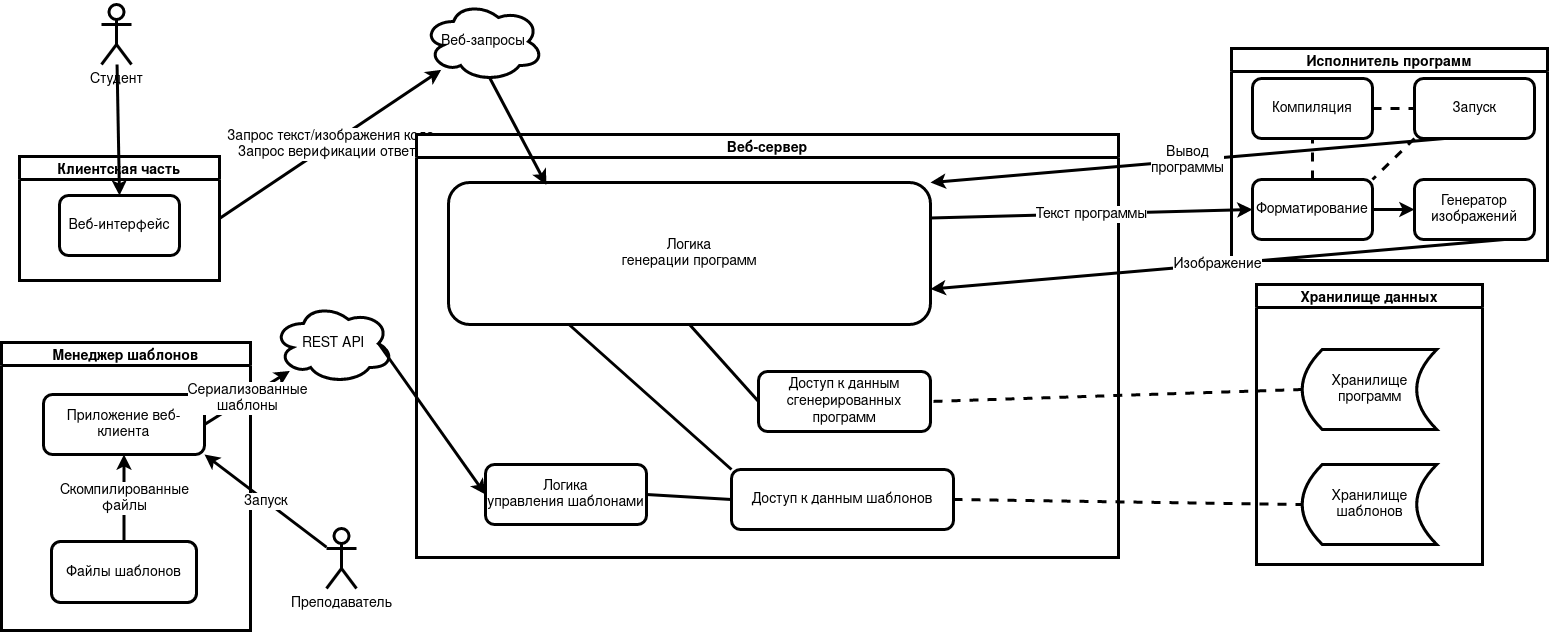
\includegraphics[width=\textwidth]{images/architecture-landscape.drawio.png}
    \end{center}
\end{frame}

\begin{frame}[fragile]
    \frametitle{Пример генерации}
    \textbf{DSL:}
    \begin{minted}[fontsize=\footnotesize]{kotlin}
val task = ProgramTemplate<PythonTag> {
    val xVar = variable("x")
    val stringLen = randomNumConstant(10, 20)
    val randomString = randomStringConstant(stringLen)
    addAssignment(xVar, randomString)
    addIfElseInstr(funcCall("len", xVar) opLt constant(15)) {
        addFuncCall("print", constant("small"))
    }.addElse {
        addFuncCall("print", constant("long"))
    }
}
\end{minted}
\end{frame}

\begin{frame}[fragile]
    \frametitle{Пример генерации}
    \textbf{Сгенерированная программа:}\\
    \begin{columns}
        \begin{column}{0.45\textwidth}
            Текст программы
            \begin{minted}[fontsize=\small]{python}
x = ".W,hHm)1^,80^6"
if len(x) < 15:
    print("small")
else:
    print("long")
            \end{minted}
        \end{column}
        \begin{column}{0.45\textwidth}
            Изображение
            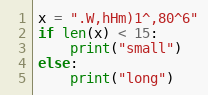
\includegraphics[width=\textwidth]{images/code-image.png}
        \end{column}

    \end{columns}
    % %     \begin{minted}[fontsize=\footnotesize]{kotlin}
    % % val task = ProgramTemplate<PythonTag> {
    % %     val xVar = variable("x")
    % %     val stringLen = randomNumConstant(10, 20)
    % %     val randomString = randomStringConstant(stringLen)
    % %     addAssignment(xVar, randomString)
    % %     addIfElseInstr(funcCall("len", xVar) opLt constant(15)) {
    % %         addFuncCall("print", constant("small"))
    % %     }.addElse {
    % %         addFuncCall("print", constant("long"))
    % %     }
    % % }
    % % \end{minted}
\end{frame}

\begin{frame}
    \frametitle{Проверка ответов}
    \begin{itemize}
        \item Запуск программы и сохранение ее вывода происходит на этапе создания кода и изображения.
        \item Сравнение ответов~--- построчно
        \item Результат проверки~--- процент правильных строк в ответе.
    \end{itemize}
\end{frame}

% \begin{frame}{Задача 2: результаты измерений в таблице}
%     \centering
%     \begin{tabular}{lccc}
%         Имя   & Работа 1 & Работа 2 & Итог \\
%         \hline\hline
%         Алиса & 8.0      & 9.0      & 8.5  \\
%         Боб   & 9.0      & 9.8      & 9.4  \\
%         Чак   & 9.1      & 9.3      & 9.2  \\
%     \end{tabular}

%     \begin{block}{Пояснения к таблице}
%         \begin{itemize}
%             \item Таблицы могут требовать пояснений.
%             \item Что это за величины? Откуда они взялись?
%             \item Какие выводы можно сделать?
%         \end{itemize}
%     \end{block}

% \end{frame}



% \begin{frame}
%     \frametitle{Задача 3: основные трудности}
%     \begin{itemize}
%         \item Мы всё классно сделали, но рецензенты STOC сформулировали ряд претензий к~работе, обозвали нас идиотами и отказались пускать на конференцию.
%         \item Все замечания были исправлены, попробуем FOCS\footnote{Не забывайте про нежелательность англицизмов и аббревиатур.}!
%     \end{itemize}

% \end{frame}

\begin{frame}
    \frametitle{Дальнейшее развитие}
    \begin{itemize}
        \item Поддержка новых элементов синтаксиса
        \item Поддержка генерации кода на других императивных языках.
        \item Интеграция в образовательные платформы (Moodle).
    \end{itemize}
\end{frame}


% \begin{frame}
%     \frametitle{Результаты работы}

%     \begin{enumerate}
%         \item Разработан полиномиальный алгоритм решения задачи коммивояжёра.
%         \item Программная реализация демонстрирует высочайшую производительность и превосходит все известные аналоги.
%         \item Результаты подготовлены для представления на~FOCS.
%     \end{enumerate}

%     \vspace{5mm}\hrule\vspace{5mm}

%     \begin{center}
%         Имя, фамилия и контакты автора,\\ссылка на материалы работы, QR-код.
%     \end{center}

% \end{frame}
\begin{frame}
    \frametitle{Результаты работы}

    \begin{enumerate}
        \item Разработан предметно-ориентированный язык для написания шаблонов программного кода.
        \item Создано приложение для генерации примеров кода для учебных задач по шаблону и параметрам
        с поддержкой проверки ответов. Данную систему можно расширять для поддержки других языков программирования.
    \end{enumerate}
        \vspace{5mm}\hrule\vspace{5mm}

    \begin{center}
        Никита Босов, \texttt{neckbosov@gmail.com},\\ \url{https://github.com/OSLL/bsc_bosov}
    \end{center}
\end{frame}

\end{document}
